\documentclass{llncs}
\usepackage{amssymb}
\usepackage[utf8]{inputenc}
\usepackage{url}
\usepackage{graphicx}
\usepackage{caption}
\usepackage{subcaption}
\usepackage{epstopdf}
\usepackage{subfig}
\usepackage{float}
\usepackage{amsmath}
\usepackage{wrapfig}
\usepackage{fancyhdr} %Usado para configurar encabezado y pie de página
\usepackage{enumitem}
%\usepackage[tight,scriptsize,centerlast]{subfigure}
\usepackage{subfloat} 
%\usepackage{subfigure}



\pagestyle{empty}
\pagestyle{fancy}
%\rfoot{\thepage}

\begin{document}

\title{Pumas@Home 2020 Team Description Paper
\thanks{Acknowledgment: This work was supported by PAPIIT-DGAPA UNAM under Grant IG100818}}
\author{
	Jesus Savage 
	\and Julio Cruz 
	\and Reynaldo Martell 
	\and Hugo Estrada 
	%\and Julio Cruz 
	\and Marco Negrete 
	\and Diego Cordero
	%\and Edgar Vazquez
	%\and Edgar Silva
	\and Manuel Pano
	\and Julio Martinez
	\and Luis Gonzalez
	%\and Luis Alvarez
	%\and Jesus Cruz
	%\and Jose Cruz
	%\and Jaime Marquez
}
\institute{Bio-Robotics Laboratory, School of Engineering \\ National Autonomous University of Mexico \\
\texttt{http://biorobotics.fi-p.unam.mx}}
\maketitle


%%%%%%%%%%%%%
%%%  ABSTRACT  %%%
%%%%%%%%%%%%%
\begin{abstract}

This paper describes the service robot Justina of team Pumas that has participated in the @Home (OPL) category of the RoboCup and RoCKIn, both of them international competitions; as well as our latest applied research. These competitions had influenced our architecture in the development of better systems for our service robots by developing algorithms to natural language understanding, semantic segemntation and Human-Robot interaction using multiple service robots.
In our robotics architecture, the VIrtual and Real roBOt sysTem (VIRBOT), the operation of service robots is divided into several subsystems, each of them has a specific functionality  that contributes to the final operation of the robot.
By combining symbolic AI with digital signal processing techniques a good performance of a service robot is obtained.

\end{abstract}

%%%%%%%%%%%%%%%
%%% INTRODUCTION %%%
%%%%%%%%%%%%%%%

\section{Introduction}

Service robots are hardware and software systems that assist humans to perform daily tasks in complex environments, to achieve this: they have to be able to understand spoken or gesture commands from humans; to be able to avoid static and dynamic obstacles while navigating in known and unknown environments; to be able to recognize and to manipulate objects and performing several other tasks that a person might request. 

Our team has been participated in the category @Home continuously since the start of this competition at the RoboCup in Bremen in 2006. Our team obtained the fourth place and got the award for the best in Speech Recognition and Natural Language Understanding in Nagoya in 2017, in the last years, in the RoboCup 2018 and 2019, the team obtained the second place.

The paper is organized as follows:
the section \ref{sec:background} enumerates the software description of our robot
Justina; the section \ref{sec:CurrentResearch}  presents  an overview of the latest research developments in our laboratory; the section \ref{sec:contributions} is about our contributions for RoboCup @Home;
in section \ref{sec:conclusions}, the conclusions and future work are given;
finally, in Appendix \ref{sec:appendix} and \ref{sec:TeamInfo}, you can find the hardware description of our robot Justina and the Information about Team Pumas.


\section{Justina's Robotics Architecture}\label{sec:background}
%\subsection{Hardware Configuration}

%Our service robot Justina, see figure \ref{fig:justina}, has the following components:\\

%\begin{wrapfigure}{r}{0.5\textwidth}
%	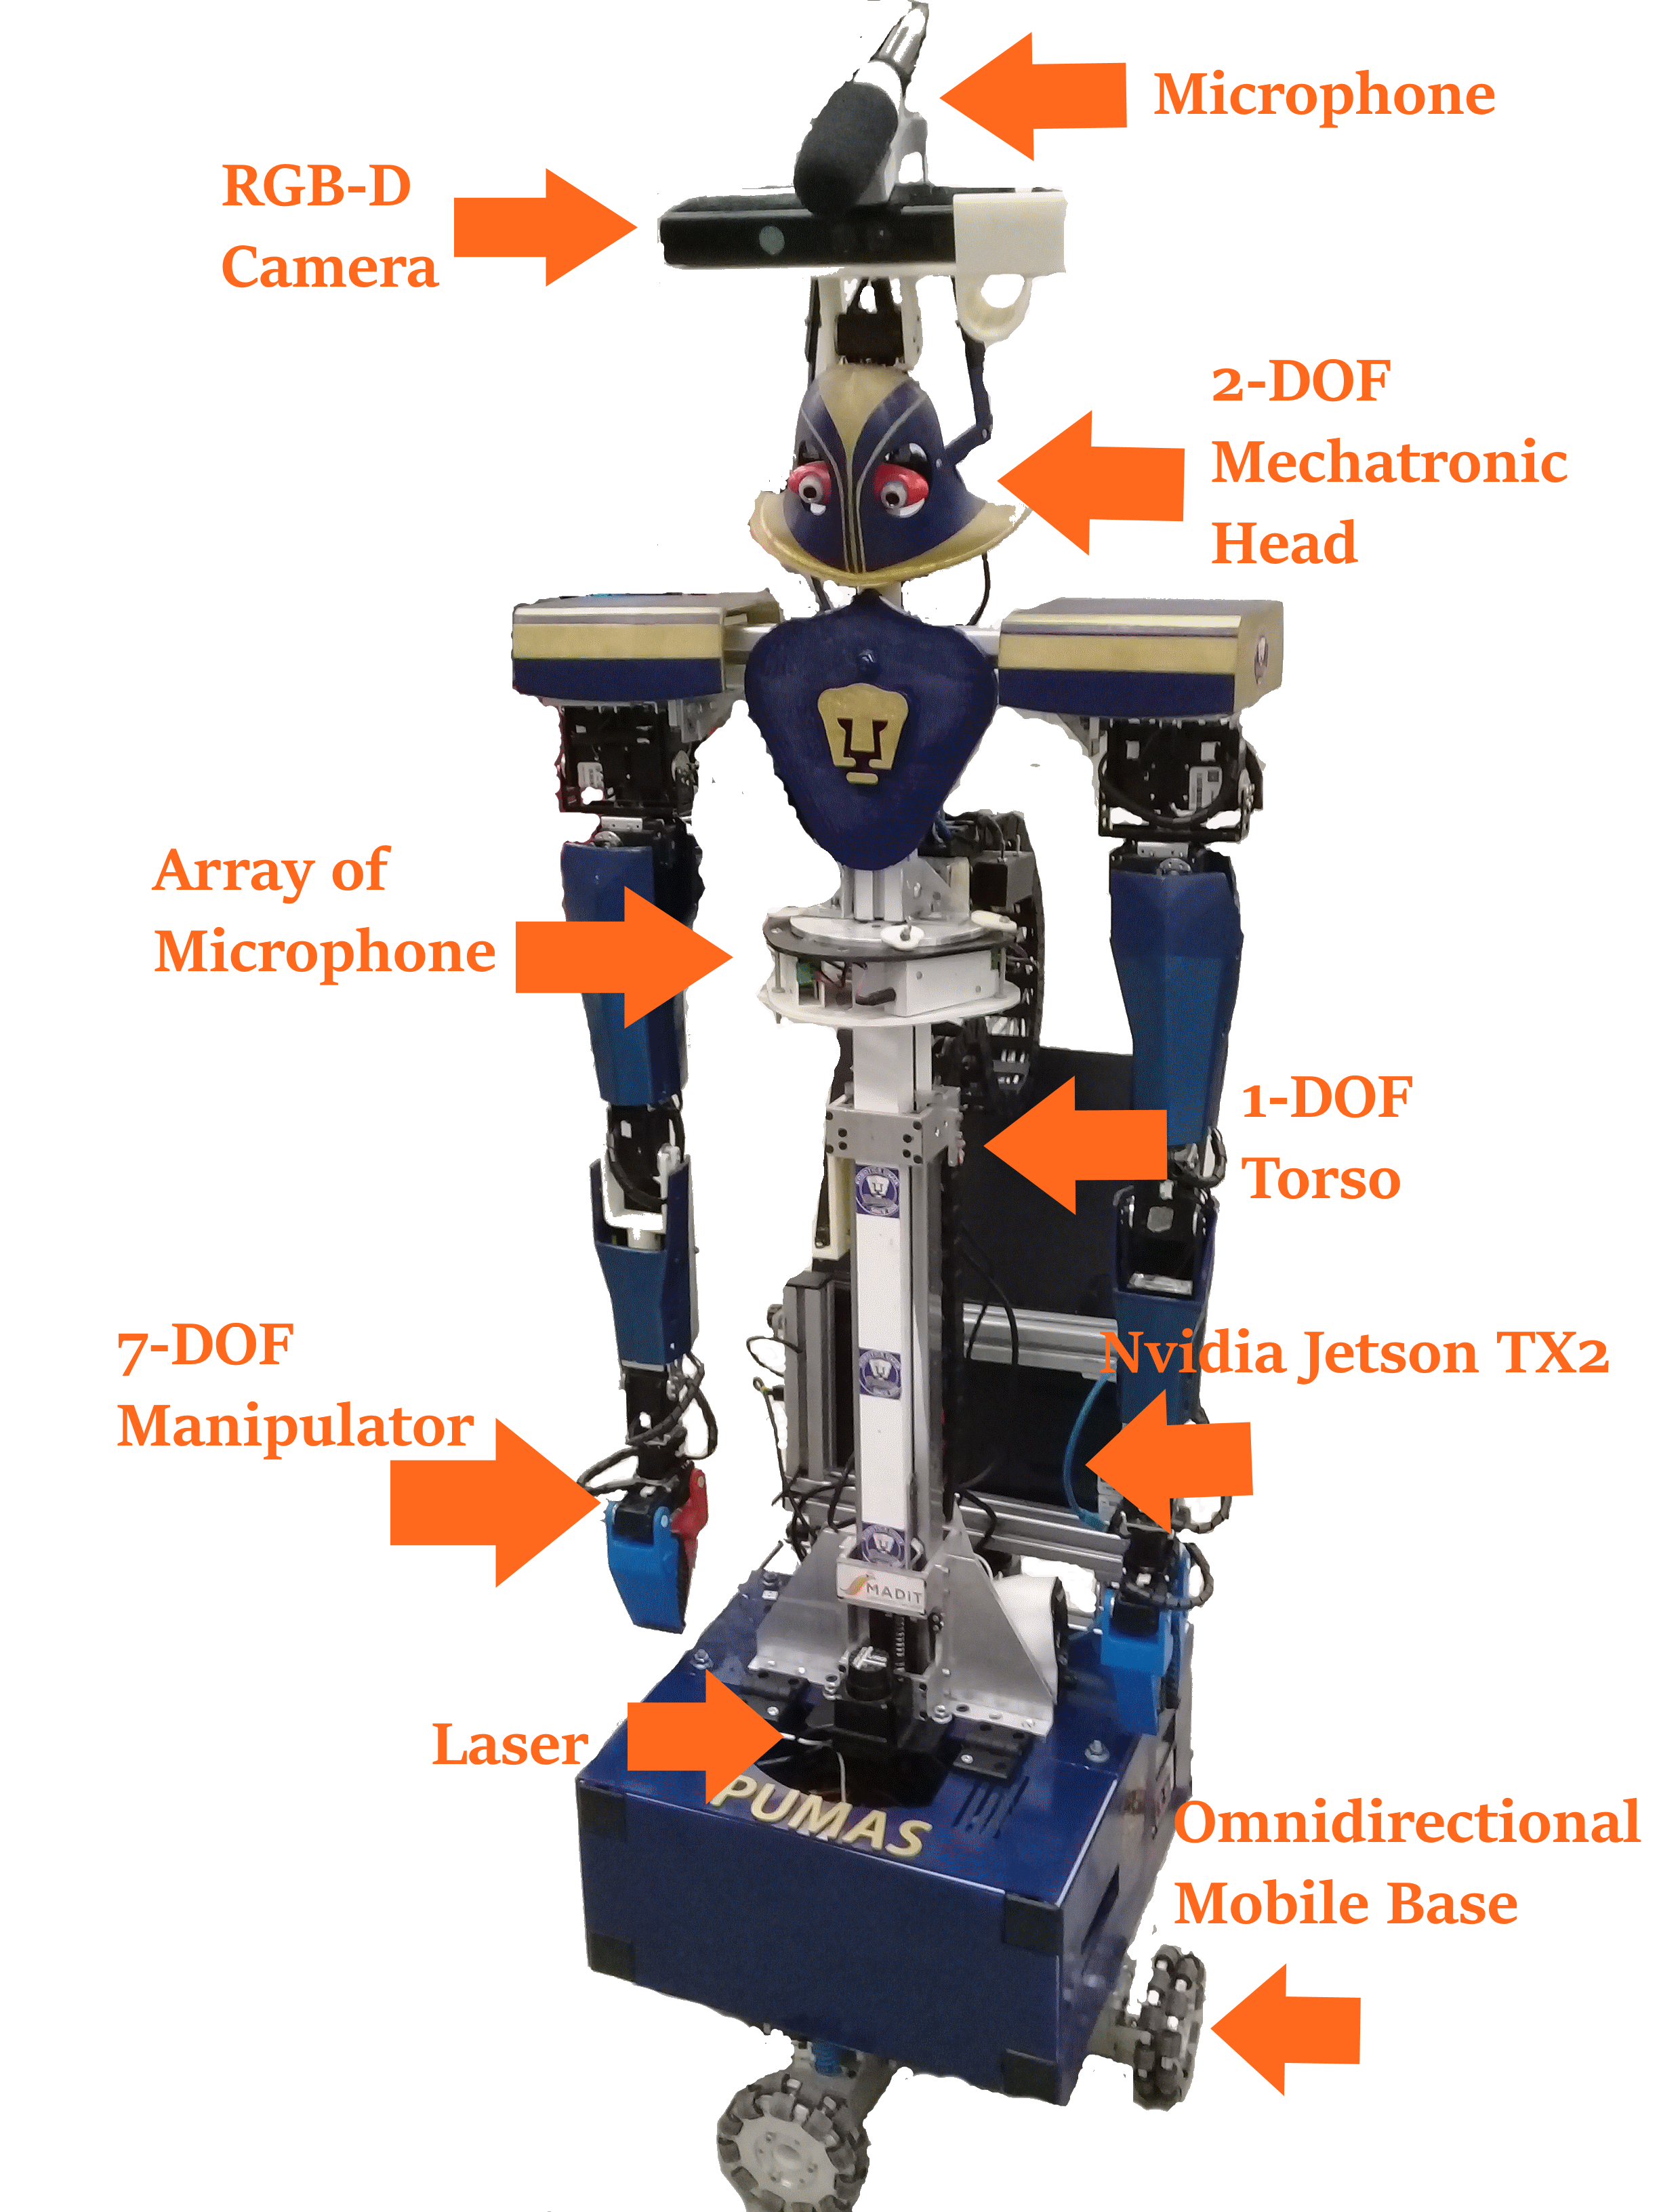
\includegraphics[angle=0, height=10.5cm, width=6.5cm]{Figures/justinaEsquema.png}
%  \caption{Robot Justina}
%  \label{fig:justina}
%\end{wrapfigure}



%HARDWARE:

%\begin{itemize}
%	\item \textbf{Mobile base:} Omnidirectional through differential pair configuration and omnidirectional wheels. 
%	\item \textbf{Manipulators:} 2 x 7-DOF anthropomorphic arms with 10 Dynamixel servomotors each.
%	\item \textbf{Head:} 2-DOF (Pan and tilt) built with Dynamixel servomotors.
%	\item \textbf{Torso:} 1-DOF (Elevation) through a worm screw and a configuration of gears. 
%	\item \textbf{Speakers:} Two speakers to generate synthetic speech.
%	\item \textbf{RGB-D Camera:} Microsoft's Kinect sensor. 
%	\item \textbf{RGB Camera:} Logitech Pro C920 Full HD.
%	\item \textbf{Microphone:} Rode NTG2 directional microphone.
%	\item \textbf{Array of Microphones:} An array of four microphones to detect sound sources.
%	\item \textbf{Laser:} Hokuyo rangefinder URG-04LX-UG0.
%	\item \textbf{Embedded System:} NVIDIA Jetson TX2 to image processing.
%\end{itemize}



\subsection{Software Configuration}
Our software configuration is based on the VIRBOT architecture \cite{virbot}, 
which provides a platform for the design and development of software for general purpose service robots, see figure \ref{fig:virbot}. 
%The VIRBOT architecture is implemented in our robots through several modules that perform well defined tasks \cite{muller}, with a high level of interaction between them. 
We use ROS as the main framework for interactuion, where a module is represented by one or 
several ROS's nodes. We use the Microsoft operating system for some modules too, besides we use our own middleware called Blackboard to link all the nodes.
In the following subsections are explained each of the layers of the VIRBOT system.


\begin{figure}[h]
	\centering
	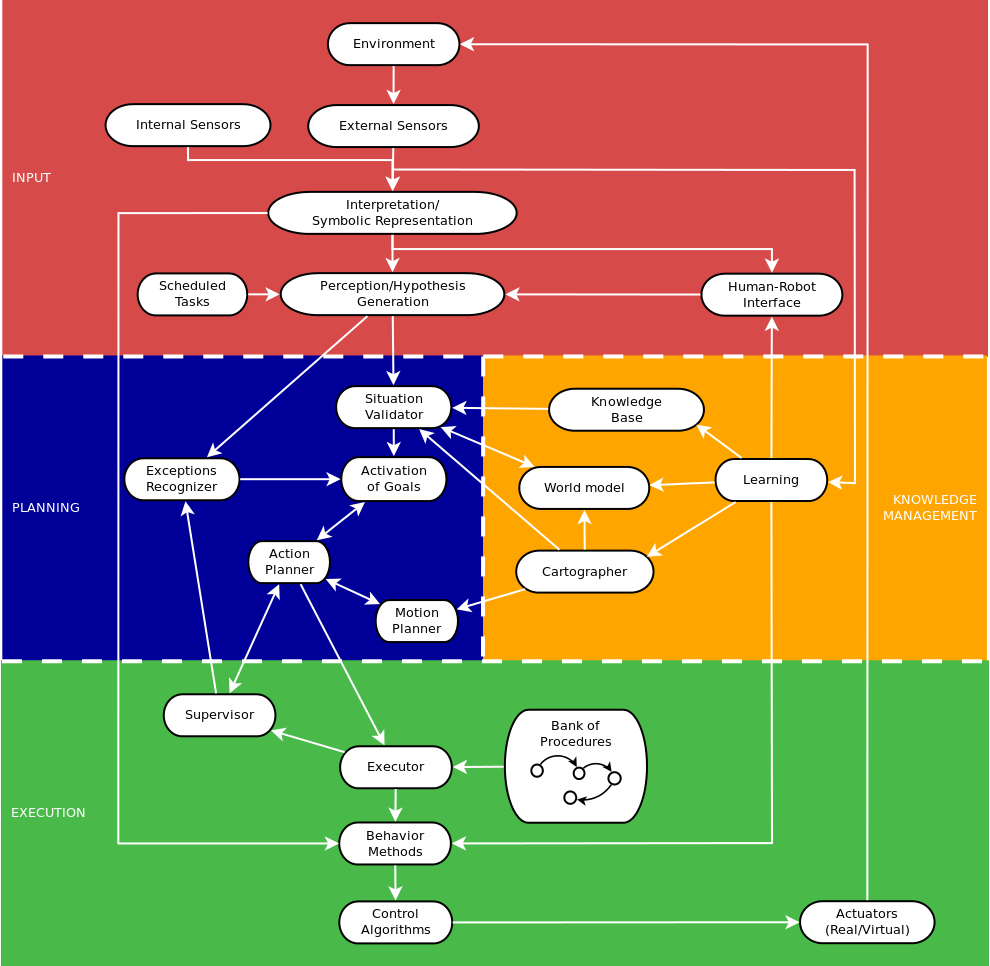
\includegraphics[angle=0, height=7.5cm, width=7.5cm]{Figures/ViRBot.png}
	\caption{Block diagram of the ViRBot architecture.}
	\label{fig:virbot}
\end{figure}


\subsection{Inputs Layer}

This layer process the data from the robot's internal and external sensors, they provide information of the internal state of the robot, along with the external world where the robot interacts.
In some of Justina's designs it has lasers, sonars, infrared, microphones and stereo and RGB-D cameras.
Digital signal processing techniques are applied to the data provided by the sensors to obtain a symbolic representation of the data, furthermore, to recognize and to process voice and visual data.
Pattern recognition techniques are used to create models of the objects and the people that interact with the robot.
Using the symbolic representation this module generates a set of beliefs, that represent the state of the environment where the robot interacts.


\subsection{Planning Layer}

The beliefs generated by the perception module are validated by this layer, it uses the Knowledge Management layer to validate them, thus a situation recognition is created. 
Given a situation recognized, a set of goals are activated in order to solve it.
Action planning finds a sequence of physical operations to achieve the activated goals.


\subsection{Knowledge Management Layer}

This layer has different types of maps for the representation of the environment, they are created using 
SLAM techniques.
Also in this layer there is a localization system, that uses the Kalman filter, to estimate the robot's position and orientation.
A rule based system, CLIPS, developed by NASA, is used to represent the robot's knowledge, in which each rule contains the encoded knowledge of an expert.


\subsection{Execution Layer}
This layer executes the actions and movements plans and it makes sure that they are executed appropriately.
A set of hardwired procedures, represented by state machines, are used to partially solve specific problems, such as, person recognition, object manipulation, etc. The action planner uses these bank of procedures and link up some of them that one may generate a plan.


%%%%%%%%%%%%%%%%%%%
%%% CURRENT RESEARCH  %%%
%%%%%%%%%%%%%%%%%%%

\section{Current research}\label{sec:CurrentResearch}
In this section is presented the current research developed in our laboratory to improve the performance of our service robots.

\subsection{Natural language understanding}\label{subsec:NaturalLU}
Natural language understanding is used in order to the service robot interprets the language and then perform an especific task.
One of the main problems using natural language understanding is the representation of meaning.  
We have a framework for defining the semantics. The robot's semantics are therefore instructions that allow it to carry out relevant operations.

Conceptual Dependency (CD) is a theory, developed by Schank \cite{Schank}, for representing the meaning contained in sentences. 
This technique finds the structure and the meaning of a sentence in just one step. 
It is useful to represent sentences using this technique when there is not a strict grammar associated with the sentences, and also when the objective is to make inferences from them.
The CD representation of a sentence is built using conceptual primitives, these represent thoughts and the relationships between thoughts. Using conceptual dependency facilitates the use of inference rules, because many inferences are already contained in the representation itself.
There are several primitives to represent actions, for example two of the more commonly used are the following:

\vspace{.01 in}
		ATRANS: Transfer of an abstract relationship (e.g., give.)

\vspace{.01 in}
		PTRANS: Transfer of the physical location of an object (e.g., go.)
\vspace{.01 in}

Each primitive represents several verbs which have similar meaning. For instance give, buy, steal, and take have the same meaning, i.e., the transference of one object from one entity to another one.
Each primitive is represented by a set of rules and data structures. Basically each primitive contains the following components:
\vspace{.01 in}

	An Actor: He is the one that perform the ACT.
\vspace{.01 in}

	An ACT: Performed by the actor, done to an object.
\vspace{.01 in}

	An Object: The action is performed on it.
\vspace{.01 in}

	A Direction: The location that an ACT is directed towards.
\vspace{.01 in}

	A State: The state that an object is in, and is represented using a knowledge base representation as
facts in an expert system. 
\vspace{.01 in}

	For instance the phrase: {\bf "Robot, please give this book to Mary"}, 
when the verb give is found in the sentence an ATRANS structure is issued.
\vspace{.01 in}

	(ATRANS (ACTOR NIL) (OBJECT NIL) (FROM NIL) (TO NIL))
\vspace{.01 in}

The empty slots (NIL) need to be filled finding the missing elements in the sentence. The actor is the robot, the 
object is the book, etc, and it is represented by the following CD:
\vspace{.01 in}

	(ATRANS (ACTOR Robot) (OBJECT book) (FROM book's owner) (TO Mary))
\vspace{.01 in}


CDs can be use for representing simple actions. It is also well suited for representing commands or simple questions, but it is not very useful for representing complex sentences.
The CD technique were implemented in an expert system.


Much of the human problem solving or cognition can be expressed by IF THEN type production rules. Each rule corresponds to a modular collection of knowledge call chunk. The chunks are organized in loose arrangement with links to related chunk of knowledge, reasoning could be done using rules. 
Each rule is formed by a left side that needs to be satisfied (Facts) and by a right side that produce the appropriate response (Actions).  
\vspace{.01 in}

		IF  Facts  THEN  Actions.
\vspace{.01 in}

When an action is issued by a rule it may become a fact for other rules, creating links to other rules. A system may use thousands of rules to solve a problem, thus it is necessary a special mechanism that will select which rules will be fired according to the presented facts. That mechanism is an Expert System "Engine".
The Inference Engine makes inferences by deciding which rules are satisfied by facts, prioritize the 
satisfied rules, and executes the rule with the highest priority.
This expert system provides a cohesive tool for handling a wide variety of knowledge with support for three different programming paradigms: rule-based, object-oriented, and procedural.
%In the VIRBOT system an expert system maintains a knowledge data base that represents the state of the world.
The data of the humans interacting with the robot, of the objects and the locations is represented using facts that contain several slots with information related with them.
The Robot is able to perform operations like grasping an object, moving itself from on place to another, finding humans, etc. Then the objective of action planning is to find a sequence of physical operations to achieve the desired goal.
These operations are represented by a state-space graph.

In the previous example, when the user says {\bf "Robot, please give this book to Mary"}: 
\begin{itemize}
\item []
	(ATRANS (ACTOR Robot) (OBJECT book) (FROM book's owner) (TO Mary))
\end{itemize}

All the information required for the actions planner to perform its operation is contained in the CD and knowledge data base. 
Our system has been described in  \cite{iros2017} and successfully tested in robotics competitions \cite{Savage}, as the RoboCup and RockIn 
\cite{Robocup_2017}, in the category @Home.
In RoboCup@Home 2017 our robot was awarded as the best in Speech and Natural Language Understanding.


\subsection{Human-Robot interaction using multiple service robots}\label{subsec:Alexa}

In our laboratory we have the vision that in the future we will not only have a service robot in our homes, 
but a variety of them performing specific tasks. The first problem to solve is find the way to communicate with all these robots regardless of where the user and the robot are.
The solution we propose is to use smart home devices to send the users requests to the service robots, see figure \ref{fig:alexahome}. 
Specifically we are using Alexa, 
the voice service that Amazon offers.

\begin{figure}[h]
	\centering
	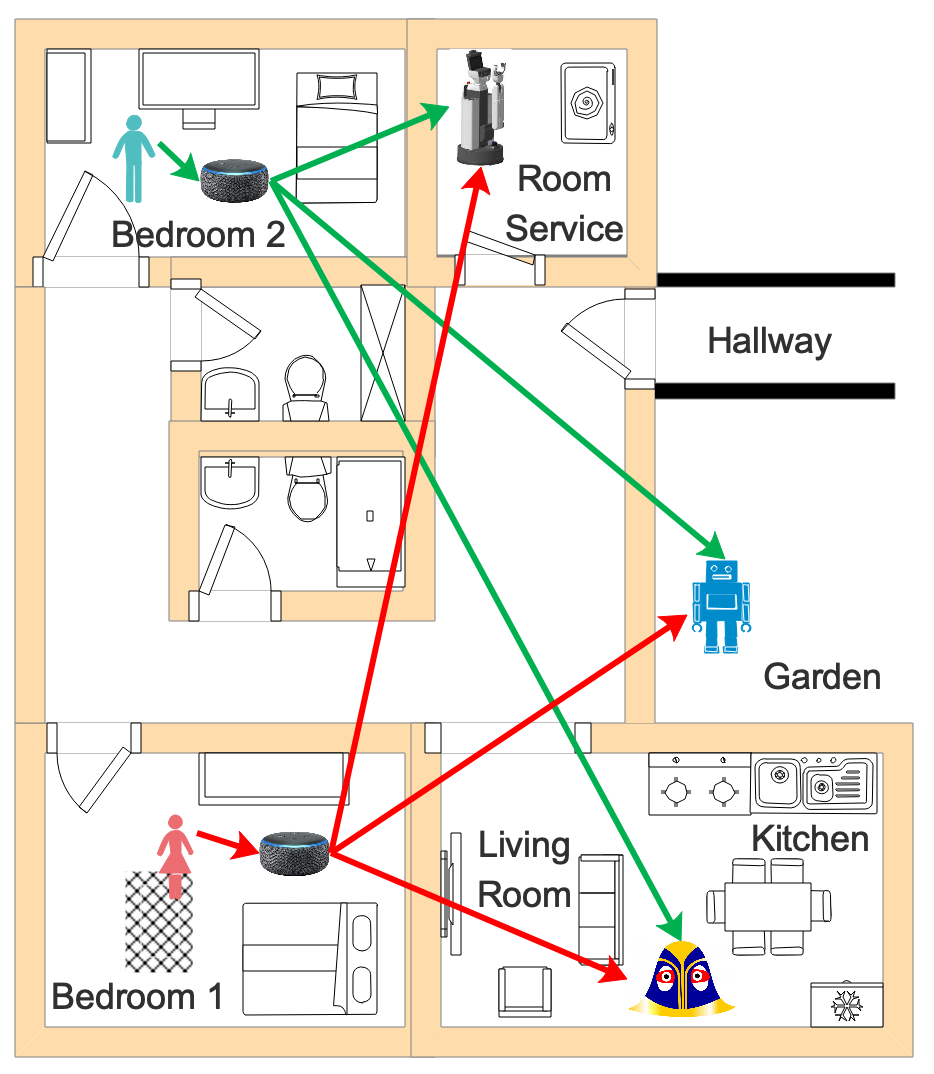
\includegraphics[angle=0, height=5cm, width=5cm]{Figures/alexa1.png}
	\caption{Human interaction with multiple robots trough intelligent devices.}
	\label{fig:alexahome}
\end{figure}

\subsubsection{Alexa integration in Justina's environment.} Alexa is an Amazon service for automatic language recognition and natural language understanding, allowing you to interact with different devices provided by this same company. However, it is also possible to extend its functionalities to third parties, so it has been possible to integrate it into the JUSTINA robot. Alexa is made up of two main elements:
\begin{itemize}
	 \item Amazon Echo - Is an array of microphones and speakers that Alexa uses as end device to be listening the user voice.
	 \item Alexa Voice Service (AVS) - Is a service for voice recognition \cite{avs}.
\end{itemize}


\subsubsection{AVS request / response handling.}

The communication between Alexa and Justina is illustrated in Figure \ref{fig:alexaconexion} and 
consists of a local area network, 
where an echo device is waiting for a user's voice command (Figure \ref{fig:alexaconexion} - 1). 
Then the voice command is sent to the AVS for recognition (Figure \ref{fig:alexaconexion} - 2), 
for a better voice recognition we use AVS's \textit{Skills} system \cite{skills}, where the \textit{Attempts} or voice commands that AVS must recognize are defined.
If AVS recognize an \textit{Attempt}, 
a request is created and sent back to the local area network (Figure \ref{fig:alexaconexion} - 3). 
To attend the request generated by AVS a web service node was created with the detail of the request (Each request is represented in a JSON format) (Figure \ref{fig:alexaconexion} - 4). 
Finally a CD, such as PTRANS or ATRANS, is generated and sent to Justina for execute the user's voice command (Figure \ref{fig:alexaconexion} - 5).
\begin{figure}[h]
	\centering
	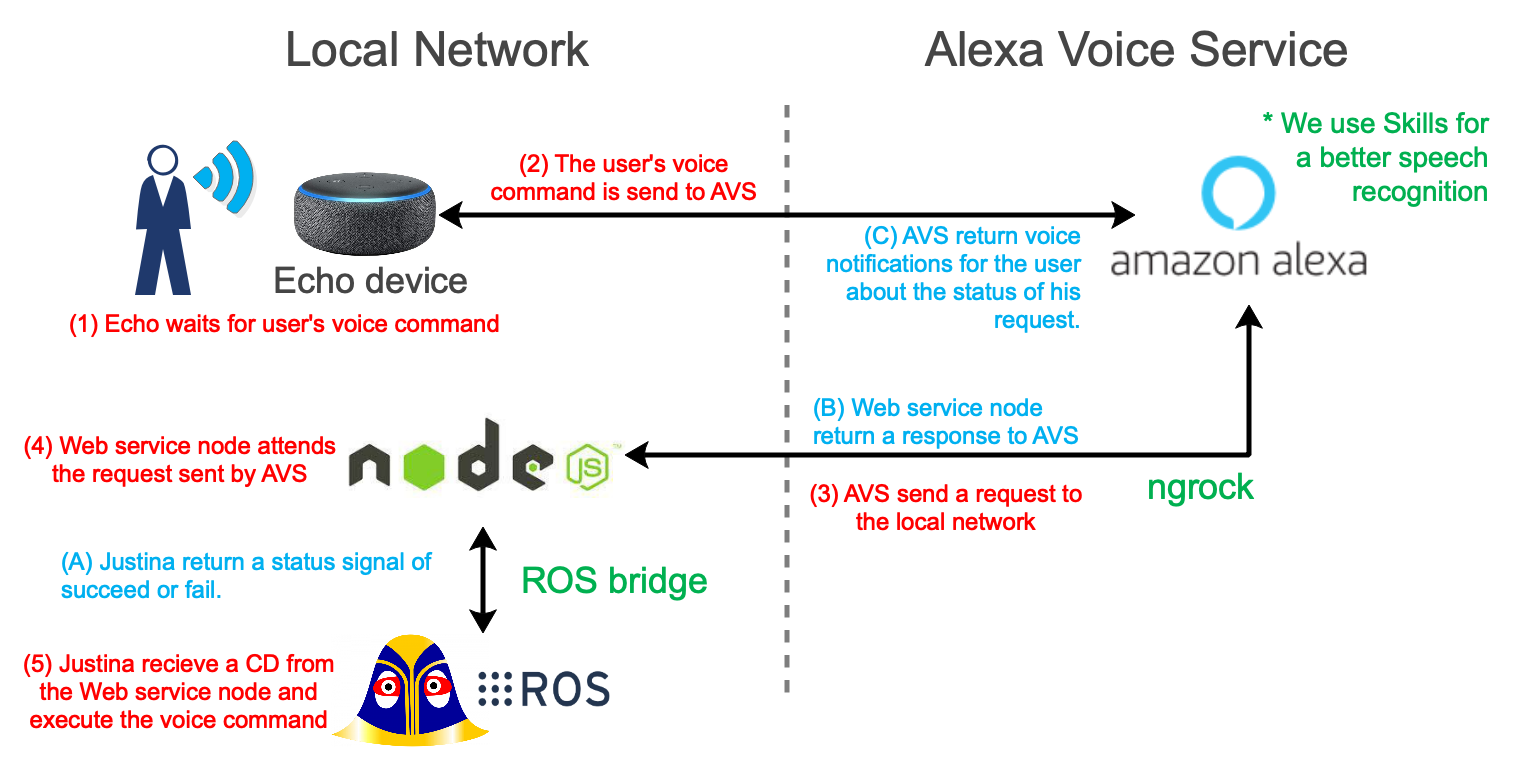
\includegraphics[angle=0, height=5cm, width=10cm]{Figures/alexa3.png}
	\caption{Block digram of Justina and alexa comunication.}
	\label{fig:alexaconexion}
\end{figure}

To use other robots through this system, a web service node must be created for each of them. 
%As in the final of RoboCup 2019, where we present Justina and Takeshi (toyota robot) working together, 
%we ask Takeshi to attend the entrance and Justina serve drinks for the guests.

%%%%%%%%%
%%% LUIS brazos 
%%% YOLO objetos sillas
%%% Torso 
%%% FaceRecog entrenar rostros y generos
%%% Monitor
%%% Reconocimiento de objetos jefe Diego
%%% P&G 
%%% alexa

%%%%
%%% Applicability of the approach in the real world
%%%%%%
\subsubsection{Applicability of the approach in the real world.} 

As previously stated, 
our vision is to have different robots inside the home performing independent or joint tasks, 
where robots can communicate with each other and with the user, 
 also robots can interact with different smart devices to perform another tasks such as turn on lights, play music, turn on appliances, open or close doors, etc.
The main purpose is to divide the work and offer to the user more options to complete the daily tasks at home.
We showed some of this work in the fnal of the RoboCup@Home Open Platform League 2019, where Justina and Takeshi worked together, in a party atmosphere, Takeshi was in charge of receiving guests at the entrance while Justina served drinks for the guests.


\subsection{Object recognition and Semantic Segmentation}\label{subsec:obj_recognition}

We are currently working on the integration of a semantic segmentation module (figure \ref{fig:semanticsegmetation}) for Justina's vision system, the main objective is to improve the object detection system.

We use a state of art convolutional neural network called Mask R-CNN \cite{mask-rcnn}, which is based on Faster R-CNN. The architecture of Mask R-CNN  is divided in four main steps; the first one, extract features applying different kernels to obtain relevant information of the images, the other three steps (prediction, bounding-box regression and  mask generation) run in parallel, all of them has the same input, a RoI (region of interest ), the feature map extracted from the first step is divided into small maps where an object of interest can be. 

\begin{figure}[h]
	\centering
	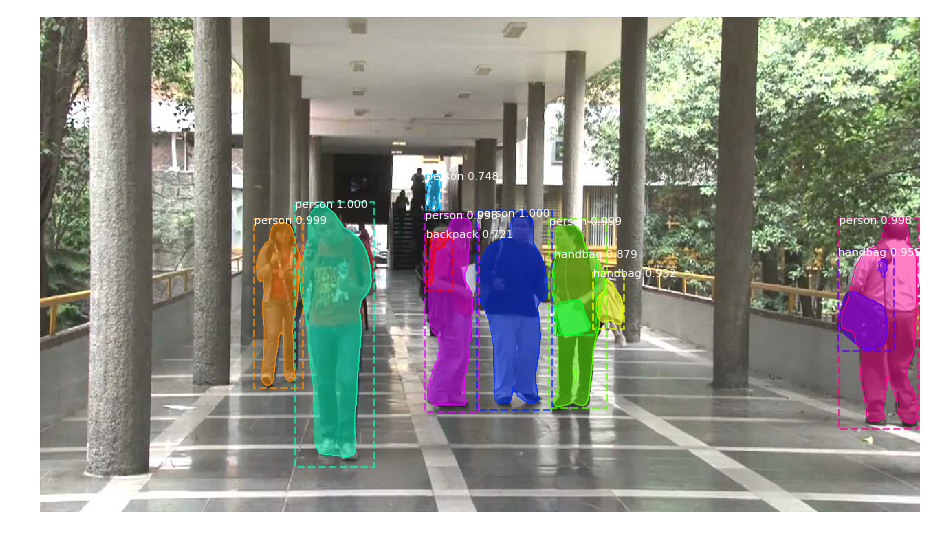
\includegraphics[angle=0, height=4cm, width=6cm]{Figures/instance_segmentation.png}
	\caption{Semantic segmentation of people scene.}
	\label{fig:semanticsegmetation}
\end{figure}

In the classification layer each RoI is flatten before to push it into the fully connected layer, the output layer is a softmax, the class of teh object is defined by the maximum output in the softmax layer. 

The mask generation step consists in generating a mask for each class in the data set and then the correct mask is chosen by the classification made by the classification step.

We use transfer knowledge and then re-training parameters of the neural network with the information of the objects we want to find in the environment of the robot.

Now we are testing different configurations in order to get a better relation between time of inference, accuracy and hardware requirements.




%%%%%%
%%% Contributions for RoboCup@Home
%%%%%%%%%
\section{Contributions for RoboCup@Home}\label{sec:contributions}
During our participation in the RoboCup@Home we have promoted, mainly in our country, 
the interest in participating and collaborating in this competition through the following contributions:

\begin{enumerate}
	\item We host the RoboCup@Home in Mexico City, Mexico, 2012.
	\item Since 2008 we have participated in the organization of Mexican Robotics Tournament (TMR) in @Home league.
	\item Extracurricular courses for programming and development of service robots, Engeneering Faculty, UNAM, 2019.
	\item Conferences at the Robotics Winter School to promote the study of robotics related topics, Xalapa Veracruz, Mexico, 2018.
	\item Outreach programs (domestic workshops, international academic exchanges, etc.) 
\end{enumerate}



%%%%%%%%%%%%%%%%%%%%%%%%%%
%%%  CONCLUSION AND FUTURE WORK  %%%
%%%%%%%%%%%%%%%%%%%%%%%%%%

\section{Conclusions and future work}\label{sec:conclusions}
We have described the main features of Justina's architecture as well as the recent research for the Robocup@Home Open Platform League 2020. Based on the performance of Justina in the competences of recent years and the state of development achieved, we improved the hardware and software systems providing our robot with better reliability and new skills to work in different environments. 
Particularly, this year, we add an Embedded Development kit \cite{jetson} to perform GPU's solutions.
In terms of software, we have change the way of conceiving the tests of the competition: passing from static state machines to inferred action planning generated by a rule based system.
We also began to develop an architecture in which different robots can communicate with each other and collaborate to help users. Moreover we are working on a CNN for semantic segmentation to boost the vision system.
The team still working to improve Justina's capabilities through the experience that RoboCup@Home have offered us since 2006.

%As for future work, we are working in a new configuration for the omnidirectional base to improve the navigation performance. Also, we will explore new topics as the memory and enviromental reasoning of the robot, in order to explain things that hapenned in the past.

%It is clear, that during the 11 years in which our team Pumas has been participated in the RoboCup and 2 years in the Rockin \cite{Robocup_2017} in the category @Home, the performance and research developed, in the service robot area, in our laboratory has been improved considerably.
%Our service robot architecture, the VIRBOT, has been evolving according to the requirements that these robotics competitions asked each year.
%In these years, the full system has been improved, both in hardware and software, having reliable performance and showing promising results. Particularly, this year, we add an Embedded Develotment kit \cite{jetson} for perform GPU's solutions.
%In terms of software, we have change the way of conceiving the tests of the competition: passing from static state machines to inferred action planning generated by a rule based system. 
%As for future work, we are working in a new configuration for the omnidirectional base to improve the navigation performance. Also, we will explore new topics as the memory and enviromental reasoning of the robot, in order to explain things that hapenned in the past.
%\bibliographystyle{unsrt}
%\bibliography{bibliography,justina}

\begin{thebibliography}{1}

\bibitem{virbot}
{\em ViRbot: A System for the Operation of Mobile Robots}, J. Savage, and et al, RoboCup 2007: Robot Soccer World Cup XI,
pp 512-519, Springer Berlin Heidelberg, 2007.

%\bibitem{muller}
%{\em The Design of Intelligent Agents: A Layered Approach}, Muller, Jorg P,Springer-Verlag New York, Inc.1997.

\bibitem{Schank}
{\em Conceptual dependency and its descendants}, S. Lytinen, Computers \& Mathematics with Applications, 1992.

\bibitem{iros2017}\textit{The Use of Expert Systems for Semantic Reasoning in Service Robots}, Jesus Savage, Julio Cruz, Reynaldo Martell, Hugo Leon, Marco Negrete, and Jesus Cruz, 2nd Workshop on Semantic Policy and Action Representations for Autonomous Robots (SPAR), IROS 2017

\bibitem{Savage}
{\em The Role of Robotics Competitions for the Development of Service Robots}, 
 Jesus Savage, Marco Negrete, Mauricio Matamoros, Jesus Cruz,
IJCAI'16, Workshop on Autonomous Mobile Service Robots, New York, USA, 2016.

\bibitem{Robocup_2017}
{\em RoboCup@Home} http://www.robocupathome.org
\\
{\em Rockin} http://rockinrobotchallenge.eu/home.php

\bibitem{avs} {\em AVS} https://developer.amazon.com/en-US/alexa/alexa-voice-service

\bibitem{skills} {\em Skills} https://developer.amazon.com/docs/ask-overviews/build-skills-with-the-alexa-skills-kit.html

%\bibitem{graspingNovelObjects}\textit{Grasping novel objects with depth segmentation}, D. Rao, Q. V. Le, T. Phoka, M. Quigley, A. Sudsang, and A. Y. Ng, 2010 IEEE/RSJInternational Conference on Intelligent Robots and Systems, pp. 2578–2585, Oct 2010.

%\bibitem{objectDetection}\textit{Object detection
%based on plane segmentation and features matching for a service
%robot}, A. J. R. Neves, R. Garcia, P. Dias, and A. Trifan, International Journal of Computer, Electrical, Automation, Control and Information Engineering, vol. 10, no. 4, pp. 775 – 782, 2016.

\bibitem{rulebook2018}\textit{Robocup@home 2018: Rules and regulations}, M. Matamoros, C. Rascon, J. Hart, D. Holz, and L. van Beek, 2018

\bibitem{mask-rcnn}\textit{Mask R-CNN}, K. He, G. Gkioxari, P. Dollár and R. Girshick, The IEEE International Conference on Computer Vision (ICCV), 2017, pp. 2961-2969

%\bibitem{iros2018}\textit{Intelligent flat-and-textureless object manipulation in Service Robots}, A. Ortega, H. Estrada, E. Vázquez, R. Martell, J. Hernández, J. Cruz, E. Silva, J. Savage, and L. Contreras, IROS 2018 Workshop "Towards Robots that Exhibit Manipulation Intelligence", 2018.

\bibitem{jetson}
{\em Jetson} https://developer.nvidia.com/embedded/buy/jetson-tx2-devkit

\end{thebibliography}

\newpage	
%%%%%%%%%%%%%%%%%%%%%%%%%%
%%%  APPENDIX  %%%
%%%%%%%%%%%%%%%%%%%%%%%%%%
\appendix
\section{Appendix}\label{sec:appendix}
\subsection{Hardware Configuration}

Our service robot Justina, see figure \ref{fig:justina}, has the following components:\\

\begin{wrapfigure}{r}{0.5\textwidth}
	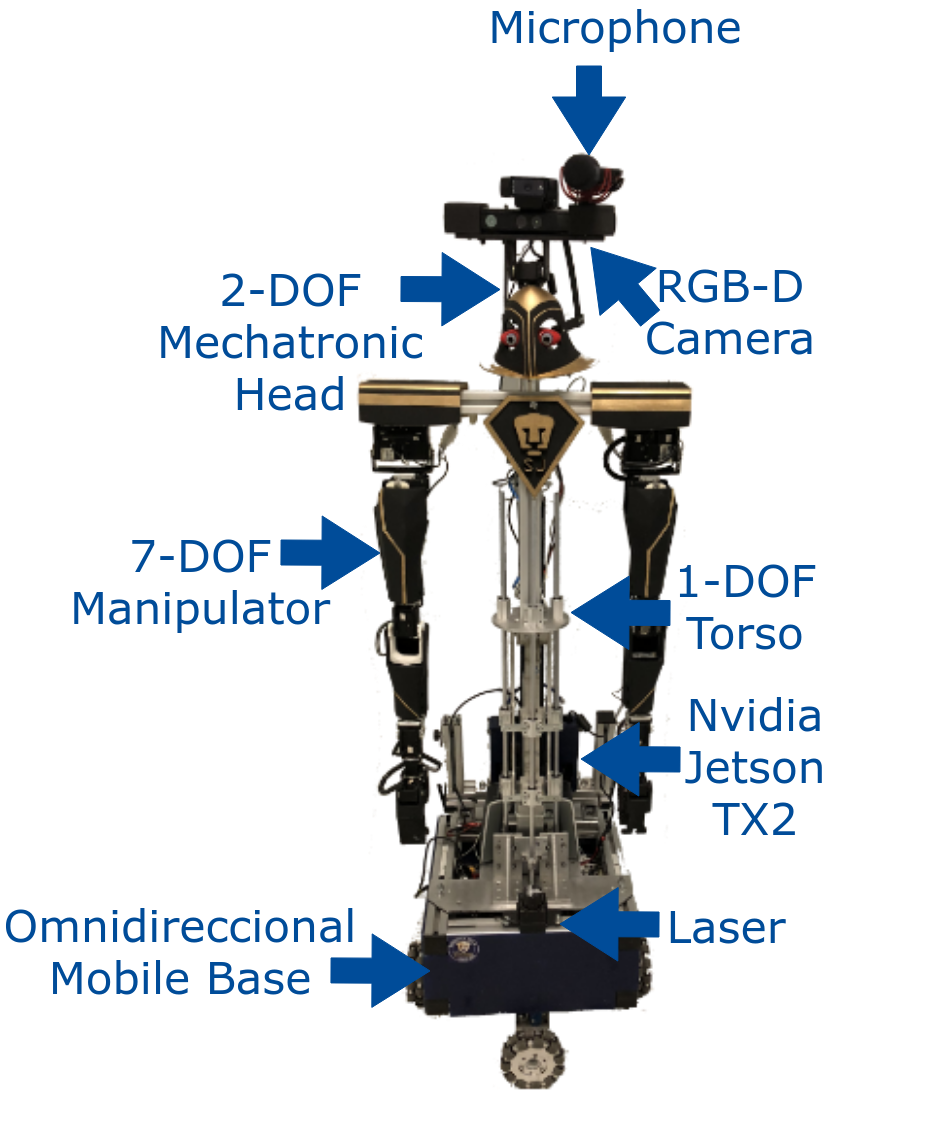
\includegraphics[angle=0, height=8.5cm, width=6.5cm]{Figures/justina_diagrama.png}
  \caption{Robot Justina}
  \label{fig:justina}
\end{wrapfigure}



HARDWARE:

\begin{itemize}
	\item \textbf{Mobile base:} Omnidirectional through differential pair configuration and omnidirectional wheels. 
	\item \textbf{Manipulators:} 2 x 7-DOF anthropomorphic arms with 10 Dynamixel servomotors each.
	\item \textbf{Head:} 2-DOF (Pan and tilt) built with Dynamixel servomotors.
	\item \textbf{Torso:} 1-DOF (Elevation) through a worm screw and a configuration of gears. 
	\item \textbf{Speakers:} Two speakers to generate synthetic speech.
	\item \textbf{RGB-D Camera:} Microsoft's Kinect sensor. 
	\item \textbf{RGB Camera:} Logitech Pro C920 Full HD.
	\item \textbf{Microphone:} Rode NTG2 directional microphone.
	\item \textbf{Array of Microphones:} An array of four microphones to detect sound sources.
	\item \textbf{Laser:} Hokuyo rangefinder URG-04LX-UG0.
	\item \textbf{Embedded System:} NVIDIA Jetson TX2 to image processing.
\end{itemize}

\newpage

\section{Team Information}\label{sec:TeamInfo}
{\bf Name of Team:} 


Pumas\\
{\bf Contact Information:}


Jesus Savage


Bio-Robotics Laboratory


Faculty of Engineering 


National Autonomous University of Mexico


robotssavage@gmail.com\\
{\bf Web Site:}


http://biorobotics.fi-p.unam.mx\\
{\bf Team Members:}


Jesus Savage, Julio Cruz, Reynaldo Martell, Hugo Estrada, Marco Negrete, 
 Diego Cordero, Manuel Pano, Julio Martinez, Luis Gonzalez\\
{\bf Hardware Description:}

Justina's Robotics Architecture (cf. Appendix A)\\
{\bf Software Description:}

Most of our software and configurations are open-source and can found at: 

https://github.com/RobotJustina/JUSTINA\\

\begin{tabular}{l@{\extracolsep{3 cm}}  r}
 \hline                 
   Operating System & Ubuntu 16.04 LTS; Windows 7 VM \\
   Middleware & ROS Kinetic; Blackboard\\
   SLAM & ROS Gmapping\\
   Navigation & Navigation using Kinect + Ocupancy grid + A*\\
   Object Recognition & Histogram Disparity + YOLO\\
   Face Detection & Haar Cascades\\
   People Detection & YOLO\\
   Gesture Recognition & OpenPoses\\
   Face Recognition & Facenet\\
   Speech Synthesis & Loquendo\\
   Speech Recognition & Microsoft Speech Recognition\\
   Inference Engine & CLIPS\\
 \hline  
 \end{tabular}

\end{document} 
